\documentclass{beamer}
\usepackage{minted}
\usepackage{hyperref}
\usepackage{xcolor}
\usetheme{metropolis}
\definecolor{cvutblue}{RGB}{1,44,86} % Defining a custom color

\setbeamercolor{palette primary}{bg=cvutblue,fg=white}
\title{Flask web evaluation for QtRvSim}
% March 16th 2024
\date{16.3.2024}
\author{Jakub Pelc}
\institute{Faculty of Electrical Engineering, Czech Technical University in Prague \par Installfest 2024}
\begin{document}
	\maketitle
	\section{Goals of this project}

	\begin{frame}{Bonus task evaluation}
		The main aim for this project is to allow external participants (as well as students) to improve their skills in computer architectures, by solving tasks in RISC-V assembly. \par

		The original way involved students of \href{https://cw.fel.cvut.cz/wiki/courses/b35apo/en/start}{\texttt{B35APO}} solving a set of \href{https://cw.fel.cvut.cz/wiki/courses/b35apo/en/homeworks/bonus/start}{\texttt{bonus tasks}},
		which were available to submit through GitLab and subsequently evaluated using \href{https://github.com/cvut/qtrvsim}{\texttt{QtRvSim}}. \par

		This is unfortunately not available to the general public, and that is the reason why this project was created.
	\end{frame}

	\begin{frame}{Current state}
		Registered users can register and submit solutions to the problems displayed on the frontpage and get immediate feedback on their solution.
		Local scoreboard is displayed for each task.\par

		This is done by running a local evaluation procedure (with the use of \href{https://github.com/cvut/qtrvsim}{\texttt{QtRvSim CLI}}), which evaluates the correctness of the code submitted and yields the performance as a score.

		The project needed to be rather simple, for it to allow easy modularity and optional modification in the future. It can be expanded by
		more features, language support, or task types. \par
		
		This is why Flask was chosen as the web framework.
	\end{frame}
	
	\begin{frame}{User interface}
		\centering
		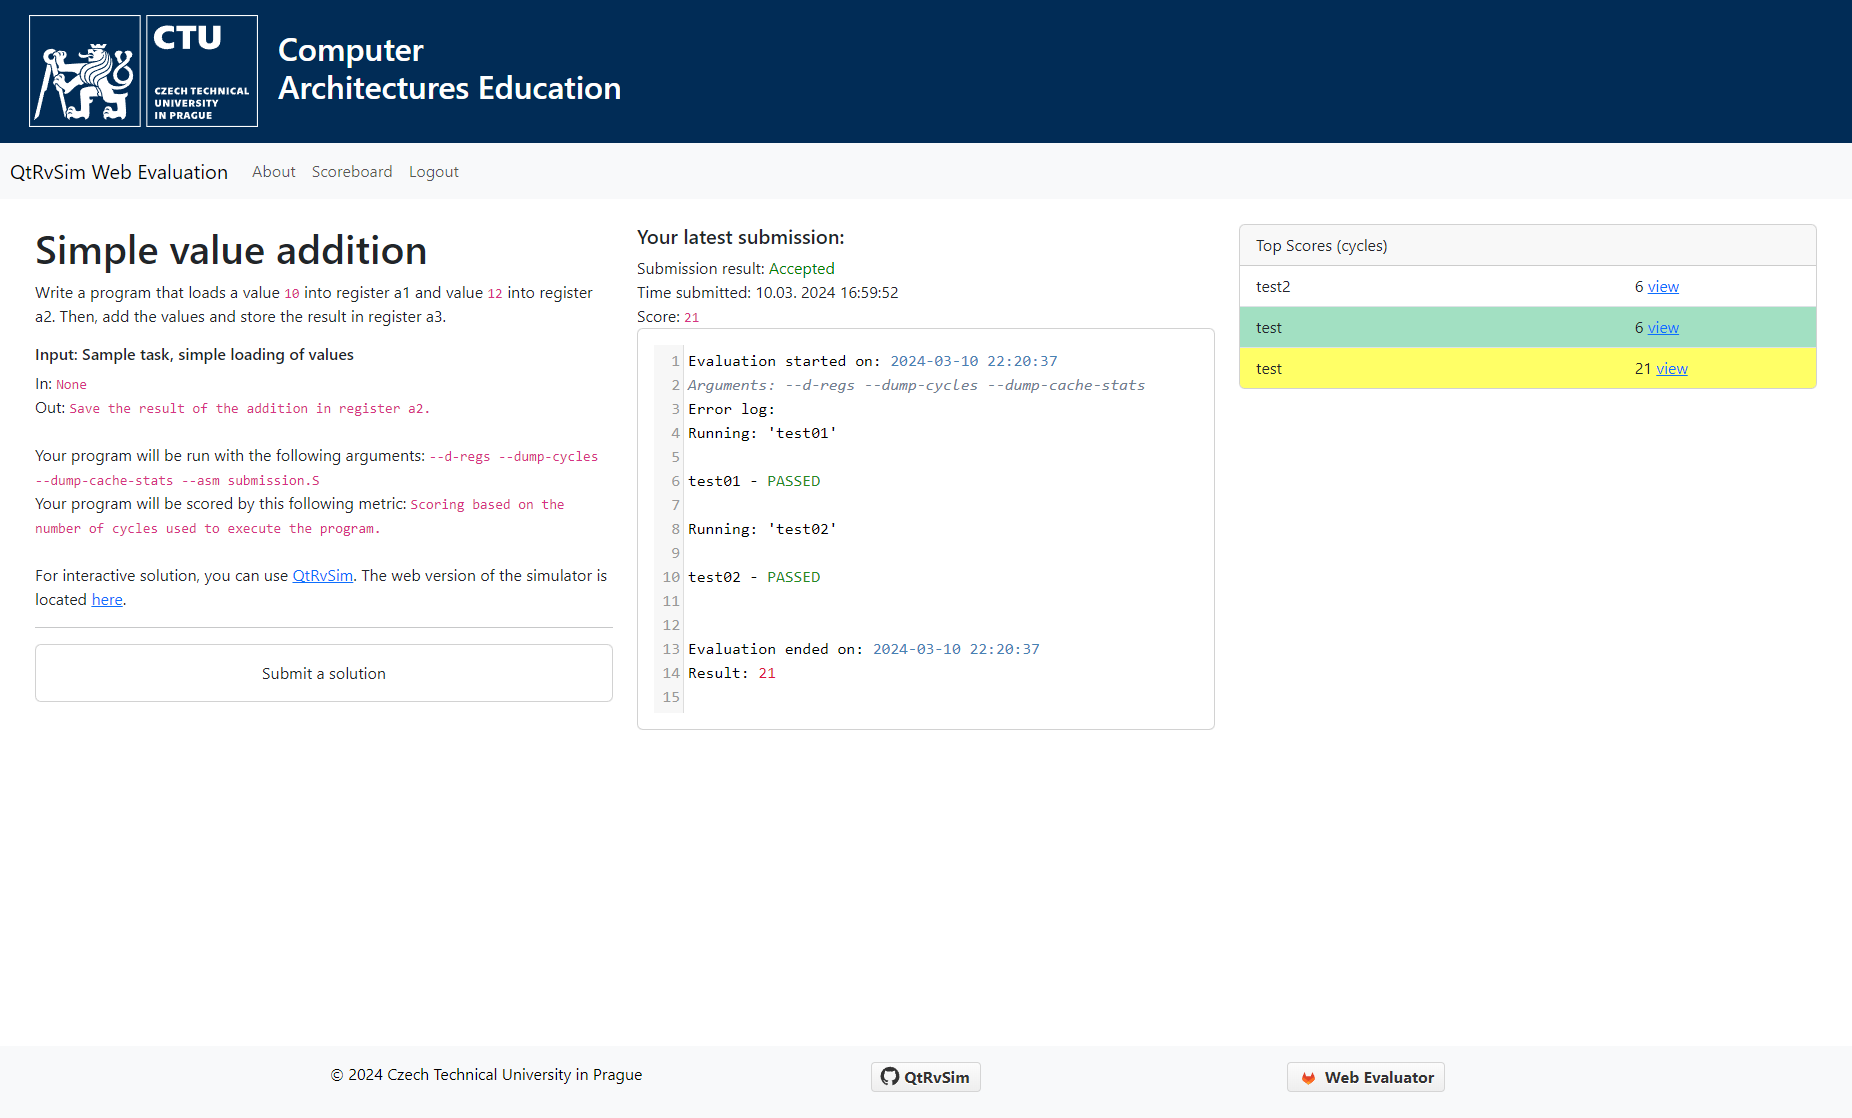
\includegraphics[width=1.0\textwidth]{images/ui.png}

		\href{http://eval.comparch.edu.cvut.cz}{\texttt{eval.comparch.edu.cvut.cz}}
	\end{frame}

	\section{A little bit about Flask}
	
	\begin{frame}{Flask}
		Flask is a micro web framework written in Python. It provides a simple way to create web applications. \par

		As opposed to Django, Flask is not an all-inclusive framework. It is designed to be simple and easy to use. \par

		To start creating a web application, the only thing needed is to have Flask installed and to have a simple python script.
	\end{frame}

	\begin{frame}[fragile]
		\begin{minted}{python}
	from flask import Flask

	app = Flask(__name__)

	@app.route("/")
	def hello():
		return "<p>Hello, World!</p>"
		\end{minted}
	\end{frame}

	\begin{frame}{Loading template files}
		We can utilize Flask to load HTML templates, instead of writing all of our HTML code in the \texttt{app.py} file. \par
		
		These template files should be located in the \texttt{templates} directory. \par

		For this example, we will use a standard HTML register page.
	\end{frame}


	\begin{frame}[fragile]
		\small
		\inputminted{python}{examples/2/app.py}
	\end{frame}

	\begin{frame}{Jinja2 templating}
		This is still not ideal, as we need to create a completely new HTML page for every route. \par

		For this problem, we can utilize the Jinja2 templating engine to create a base template, and then inherit from this template.

		Static files (such as CSS stylesheets, or images) can also be included. \par
	\end{frame}

	\begin{frame}[fragile]
		\tiny
		\inputminted{html}{examples/3/templates/base.html}
	\end{frame}

	\begin{frame}[fragile]
		\small
		\inputminted{html}{examples/3/templates/register.html}
	\end{frame}

	\begin{frame}{Flask sessions}
		The session system allows the storage of information about the user across multiple requests. \par

		Variables can also be passed to the template which are then used while rendering the page. \par

		This can be demonstrated by creating a simple login system.
	\end{frame}


	\begin{frame}[fragile]
		\tiny
		\inputminted{python}{examples/4/app.py}
	\end{frame}

	\section{Database}

	\begin{frame}{Communication with the database}
		In the web application, a PostgreSQL database is used. \par

		Only a few tables are needed to store the information about the users, tasks, submissions and results. \par

		PostgreSQL triggers are used to automatically update the best score and source code. 
	\end{frame}

	\begin{frame}{Users Table}
		\centering
		\begin{tabular}{|l|l|l|l|}
		\hline
		Field & Type & Length & Default \\
		\hline
		id & int & 32 & AUTO\_INCREMENT \\
		username & varchar & 128 & None \\
		password & varchar & 128 & None \\
		email & varchar & 128 & None \\
		salt & varchar & 128 & None \\
		verification\_code & varchar & 128 & None \\
		user\_verified & tinyint & 1 & 0 \\
		\hline
		\end{tabular}
	\end{frame}

	\begin{frame}{GDPR}
		Email adresses of the users are not being saved (due to GDPR), but during the registration process, the users are required to provide an email address for verification purposes. So how is that achieved?\par

		The email address is saved as a salted \texttt{SHA-256} hash. This way, the email address can we verified, but cannot be reverse engineered to obtain the original email address. \par

		This also allows for password reset functionality, without the need to store the email address in a readable format. Users always need to provide the email address, which is then checked against the hash in the database.
	\end{frame}

		\begin{frame}{Submissions Table}
			\centering
			\begin{tabular}{|l|l|l|l|}
			\hline
			Field & Type & Length & Default \\
			\hline
			id & int & 64 & AUTO\_INCREMENT \\
			userid & int & 64 & None \\
			taskid & int & 64 & None \\
			file & text & 64 & None \\
			evaluated & tinyint & 1 & 0 \\
			time & datetime & None & current\_timestamp() \\
			\hline
			\end{tabular}
		\end{frame}

		\begin{frame}{Results Table}
			\small
			\centering
			\begin{tabular}{|l|l|l|}
			\hline
			Field & Type & Default \\
			\hline
			userid & bigint & PRIMARY \\
			taskid & bigint & PRIMARY \\
			result\_file & text & NULL \\
			last\_source & text & NULL \\
			best\_source & text & NULL \\
			score\_last & integer & -1 \\
			score\_best & integer & -1 \\
			time & timestamp with time zone & CURRENT\_TIMESTAMP \\
			result & smallint & -1 \\
			\hline
			\end{tabular}
		\end{frame}

		\begin{frame}[fragile]
			\begin{minted}{python}
import psycopg2
import os

db_config = {
	'user': os.getenv('DB_USER'),
	'password': os.getenv('DB_PASSWORD'),
	'host': os.getenv('DB_HOST'),
	'database': os.getenv('DB_DATABASE'),
	'port': os.getenv('DB_PORT'),
	'sslmode': 'require',
	'connect_timeout': 10
}
			\end{minted}
		\end{frame}

		\begin{frame}[fragile]
			\begin{minted}{python}

def connect():
	db = psycopg2.connect(**db_config)
	cursor = db.cursor()
	return (db, cursor)

def get_user(username):
  (db, cursor) = connect()
  cursor.execute('SELECT password FROM \
	users WHERE username = %s', (username,))
  user = cursor.fetchone()
  cursor.close()
  db.close()
  return user
	
			\end{minted}
		\end{frame}

		\section{Evaluation using QtRvSim}

		\begin{frame}{Submission evaluation}
			Each of the submissions is being evaluated by a \texttt{qtrvsim\_cli} python 
			wrapper \href{https://gitlab.fel.cvut.cz/b35apo/qtrvsim-eval-web/-/blob/main/evaluator/qtrvsim.py}{\texttt{qtrvsim.py}}. \par
	
			For each task, a \texttt{.toml} file defines its structure, this file is then parsed using an \href{https://gitlab.fel.cvut.cz/b35apo/qtrvsim-eval-web/-/blob/main/evaluator/evaluator.py}{\texttt{evaluator.py}} script. A new QtRvSim instance is initialized with needed parameters,
			the instance evaluates all the testcases declared in the task file and measures the performance of the user's submission. \par
	
			The result, score, and the log are then displayed to the user.
		\end{frame}
	
		\begin{frame}[fragile]
			\tiny
			\inputminted{python}{examples/5/evaluate.py}
		\end{frame}

		\begin{frame}[fragile]
			\tiny
			\inputminted{toml}{examples/5/task.toml}
		\end{frame}

		\begin{frame}{Advanced tasks}
			The evaluator is also able to set a cache for the task, whose parameters are configurable as a part of the task. This is done by setting the maximum cache size for the task, users are then required to configure the cache parameters. \par

			Serial input and output can also be used. \par

			It is also possible, to create a task in \texttt{C}, but this also requires a custom Makefile to be provided in the taskfile. If custom files need to be present at compile time, they can also be provided. \par
		\end{frame}

		\begin{frame}[fragile]
			\small
			\inputminted{toml}{examples/5/cache.toml}
		\end{frame}

		\begin{frame}[fragile]
			\tiny
			\inputminted{toml}{examples/5/complex.toml}
		\end{frame}

	\section{Mini Competition}

	\begin{frame}{Mini Competition}
		On the page \par
		{\centering \texttt{\href{http://eval.comparch.edu.cvut.cz}{eval.comparch.edu.cvut.cz}} \par}
		you can try out your skills in RISC-V assembly. \par

		For each task the best five users will acquire $(6 - p)$ points, where p is the place they finished (according to the cycles needed to execute their solution).\par
		
		If two users finish with the same amount of cycles, their solution will be scored with the higher amount of points. \par

		We offer FEE CTU merch for the best users overall, who submit their solutions before 17.3. 12:45. \par
	\end{frame}

	\section{References}

	\begin{frame}{References}
		Links and references: \par
		{\centering \texttt{\href{https://flask.palletsprojects.com/en/3.0.x/}{Flask}} \par}
		{\centering \texttt{\href{http://eval.comparch.edu.cvut.cz}{eval.comparch.edu.cvut.cz}} \par}
		{\centering \texttt{\href{http://comparch.edu.cvut.cz}{comparch.edu.cvut.cz}} \par}
		{\centering \texttt{\href{https://github.com/cvut/qtrvsim}{QtRvSim repository}} \par}
		{\centering \texttt{\href{https://gitlab.fel.cvut.cz/b35apo/qtrvsim-eval-web}{Web Eval repository}} \par}
		{\centering \texttt{\href{https://github.com/kubakubakuba/if24-flask-web-eval}{Slides with examples}} \par}
		{\centering \texttt{\href{https://swpelc.eu}{Jakub Pelc}} \par}
	\end{frame}

\end{document}